% !TEX root = sum1.tex

\section{Results}

% The nested structure makes the greedy method useful.
% Remark: Similar to what we mentioned, the greedy method refers to using the largest groups to fill the seats.

% For M2, Merit: The plan will be always feasible. Demerit: Cannot cover all possible demands.
% Improvement:
% For $\X^{0}$, we introduce one empty seat, $x_1$. But it cannot provide the feasibility.


\subsection{Different probabilities}
Discuss the effect of different probabilities.
$E(D) = (p_1 * 1 + p_2 * 2 + p_3 * 3 + p_4 * 4) T$

% When $p = [0.25, 0.25, 0.25, 0.25]$, $E(D) = 2.5 T$. Let $p_1*1 + p_2*2 + p_3*3 + p_4*4 = 2.5$, 
% Let $E(D) = 150, T = 50, 60, 75$. The number of seats: 200, 210, 225.

% 1: When $E(D)$ is fixed, case3,4 need a larger hall to accept the same number of people.

% Different layout may make a difference.

% 2. The assumption that $T$ is fixed will be more reasonable for the continuous time. 

Let $E(D) = 150$.

Two experiments:
When $E(D) = 2.5T$, which means on average 2.5 people arrive for each group.

$T =75$, the number of rows is 9, the number of seats each row is 25.

Probabilities: 
$p_1 = p_3 + 2p_4$. $p_3$ is from $0.05$ to $0.45$ with step size of 0.1. $p_4$ is from $0.05$ to $0.3$ with step size of 0.05.

Results: M1-M6, the number of accepted people, the number of total people.

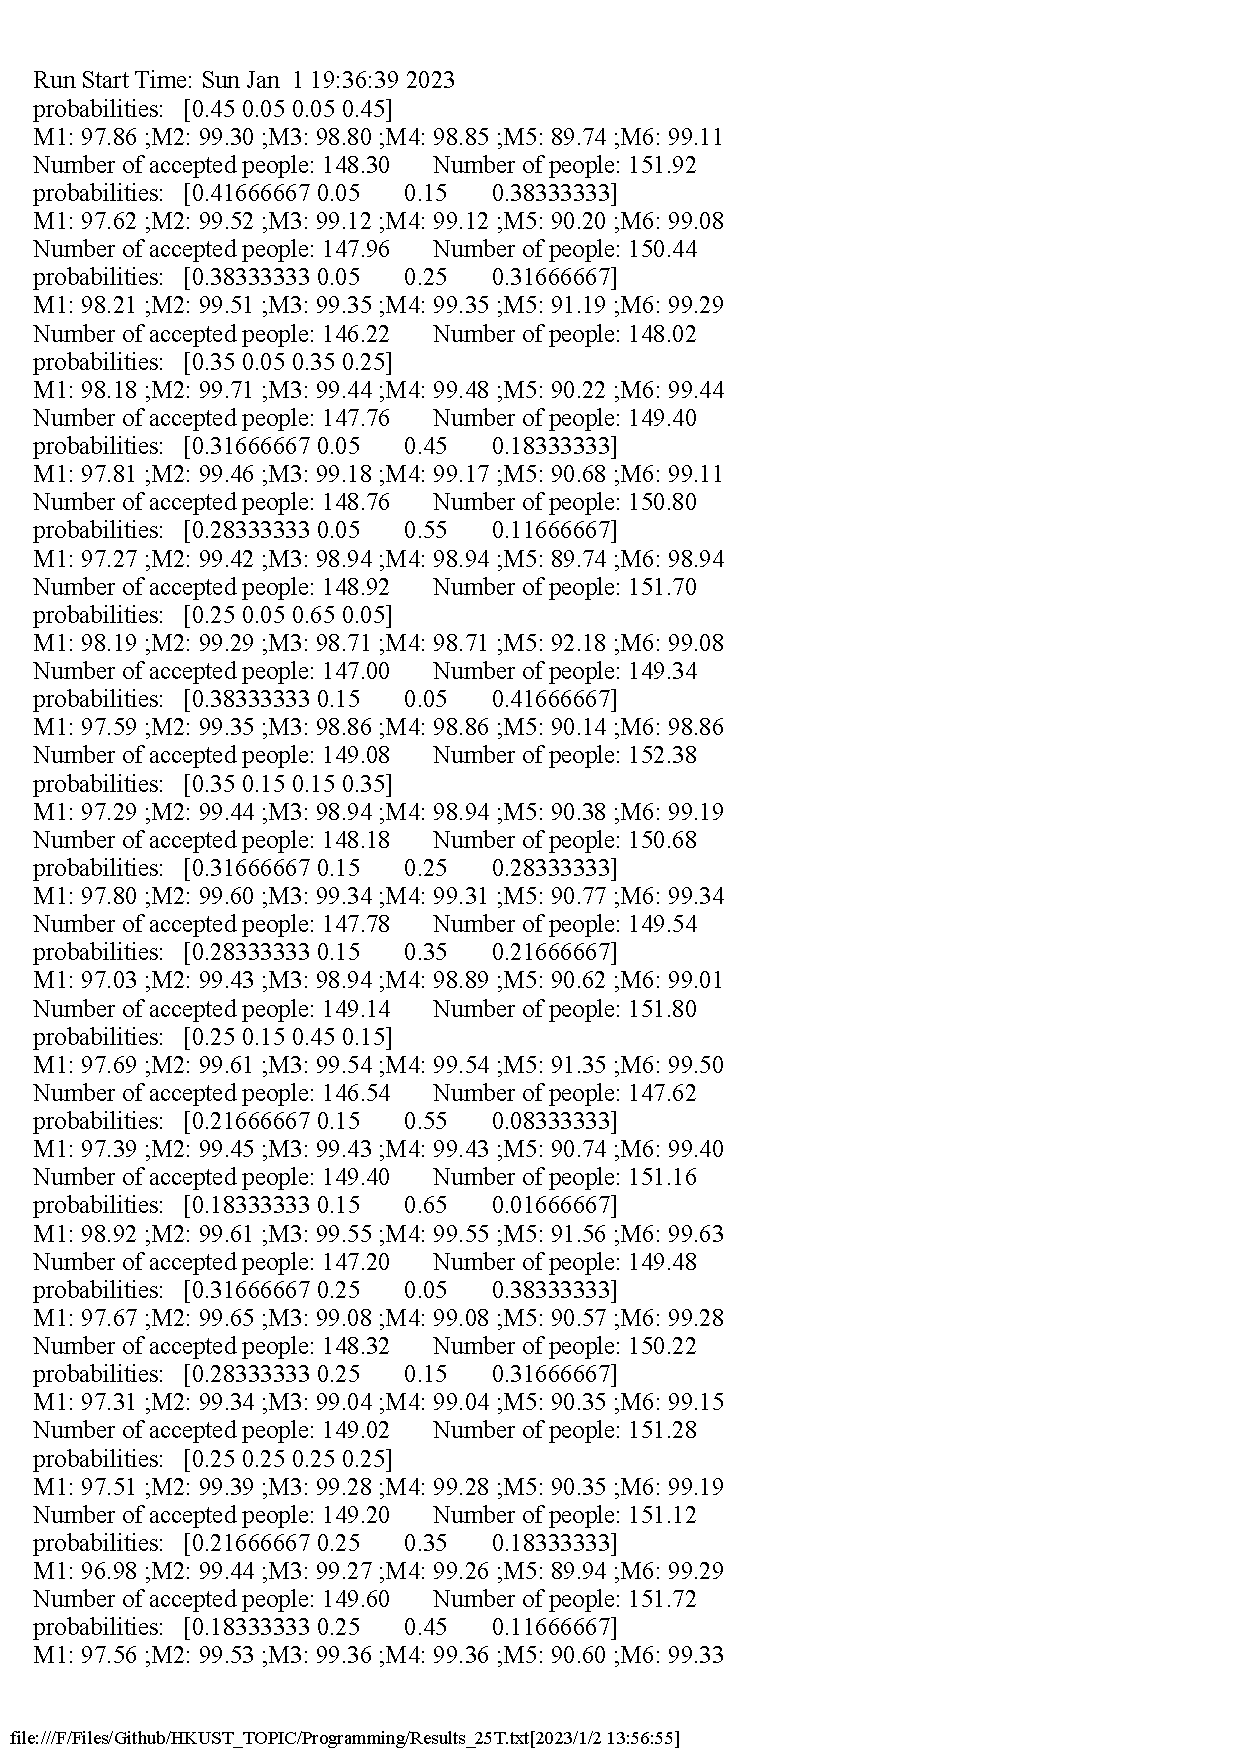
\includepdf{./Figures/Results_25T.pdf}

When $E(D) = 2T$, which means on average 2 people arrive for each group.

$T = 60$, the number of rows is 10, the number of seats each row is 21.

Probabilities: 
$2p_2 + 4p_3 + 6p_4 =3$. $p_2$ is from $0.05$ to $0.95$ with step size of $0.1$. $p_3$ is from $0.05$ to $0.75$ with step size of $0.1$.

Results: M1-M6, the number of accepted people, the number of total people.

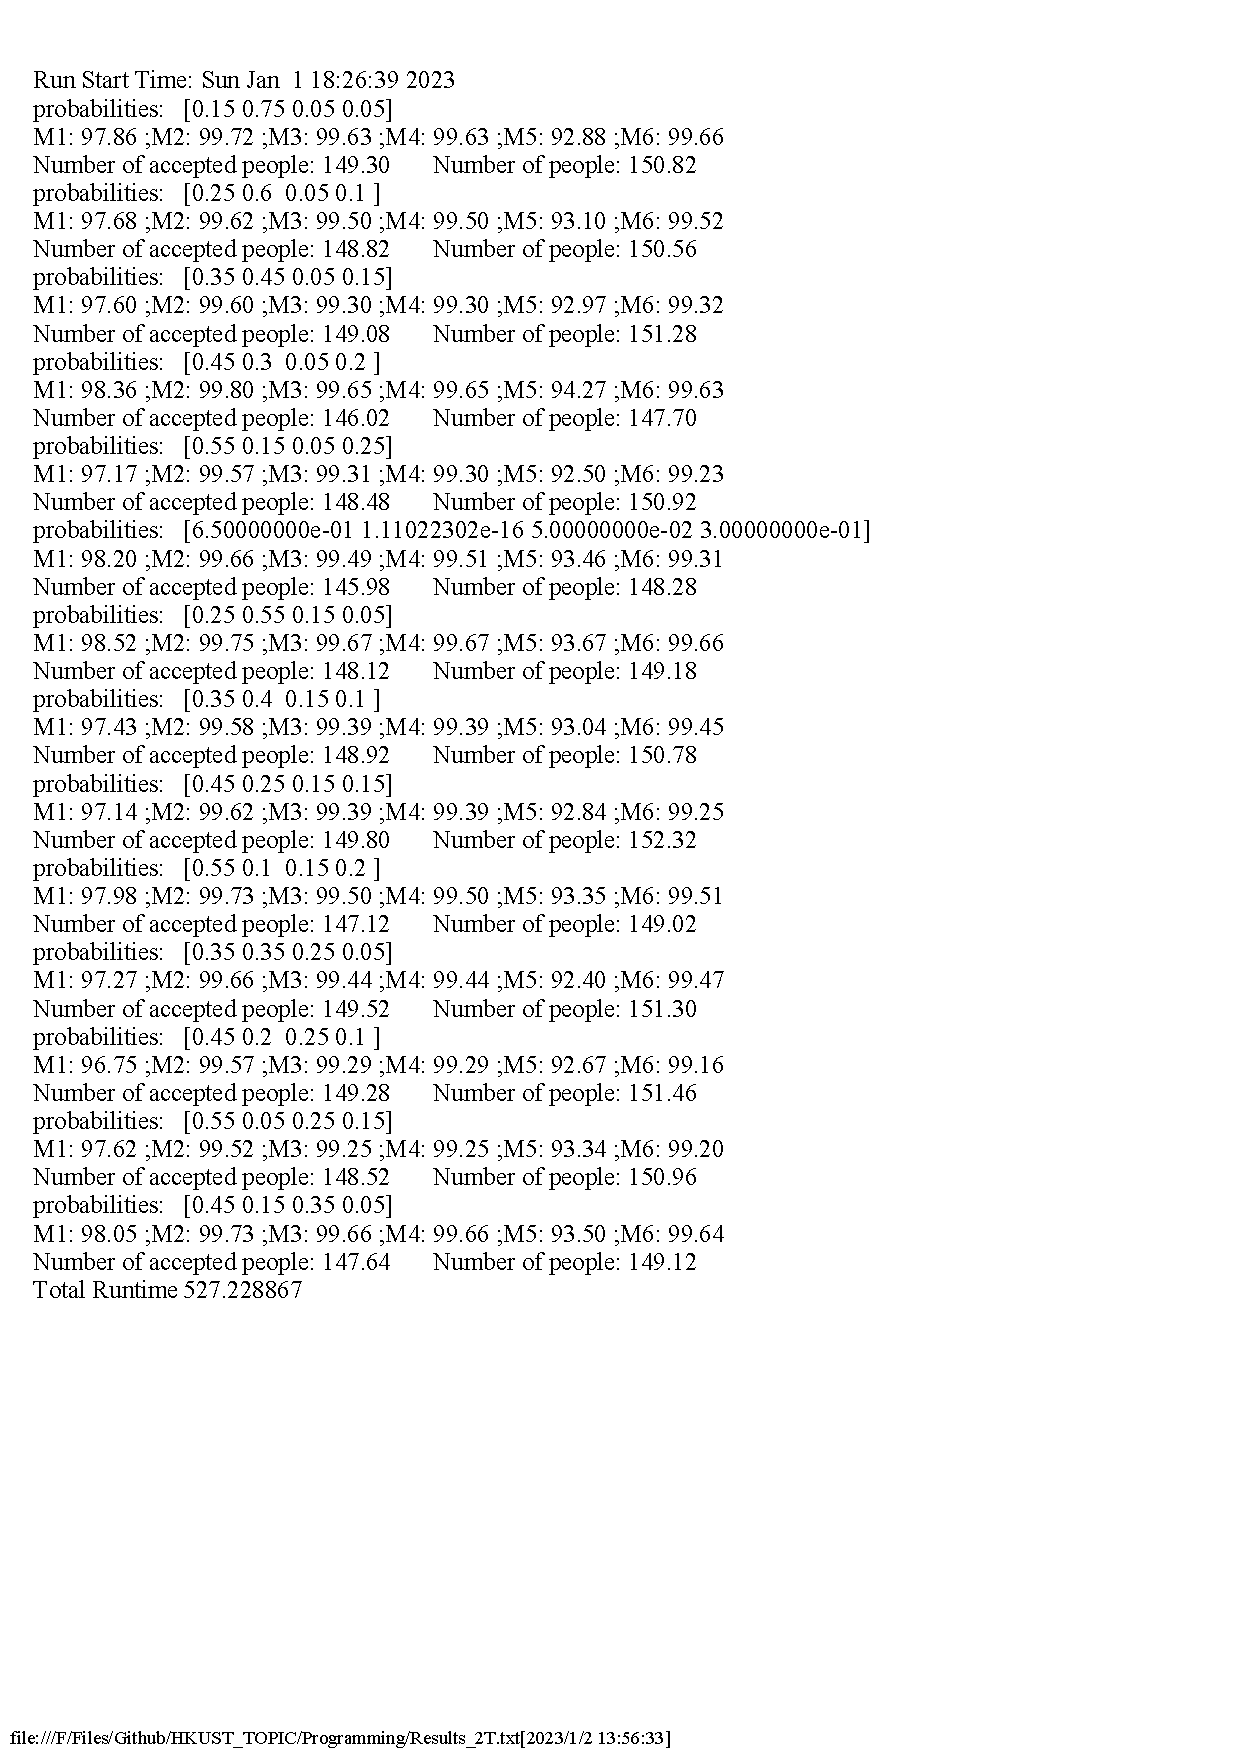
\includepdf{./Figures/Results_2T.pdf}

\subsection{Different periods}
Discuss the effect of the number of periods: 
Parameters: T = 70-80, step size =1.

The expected number of period: 75
The expected number of demand(people): 150
Number of rows: 9
Number of seats each row: 25
Probabilities: $[0.4, 0.3, 0.2, 0.1], [0.3, 0.5, 0.1, 0.1]$.

Results: M1-M6, the number of accepted people, the number of total people.

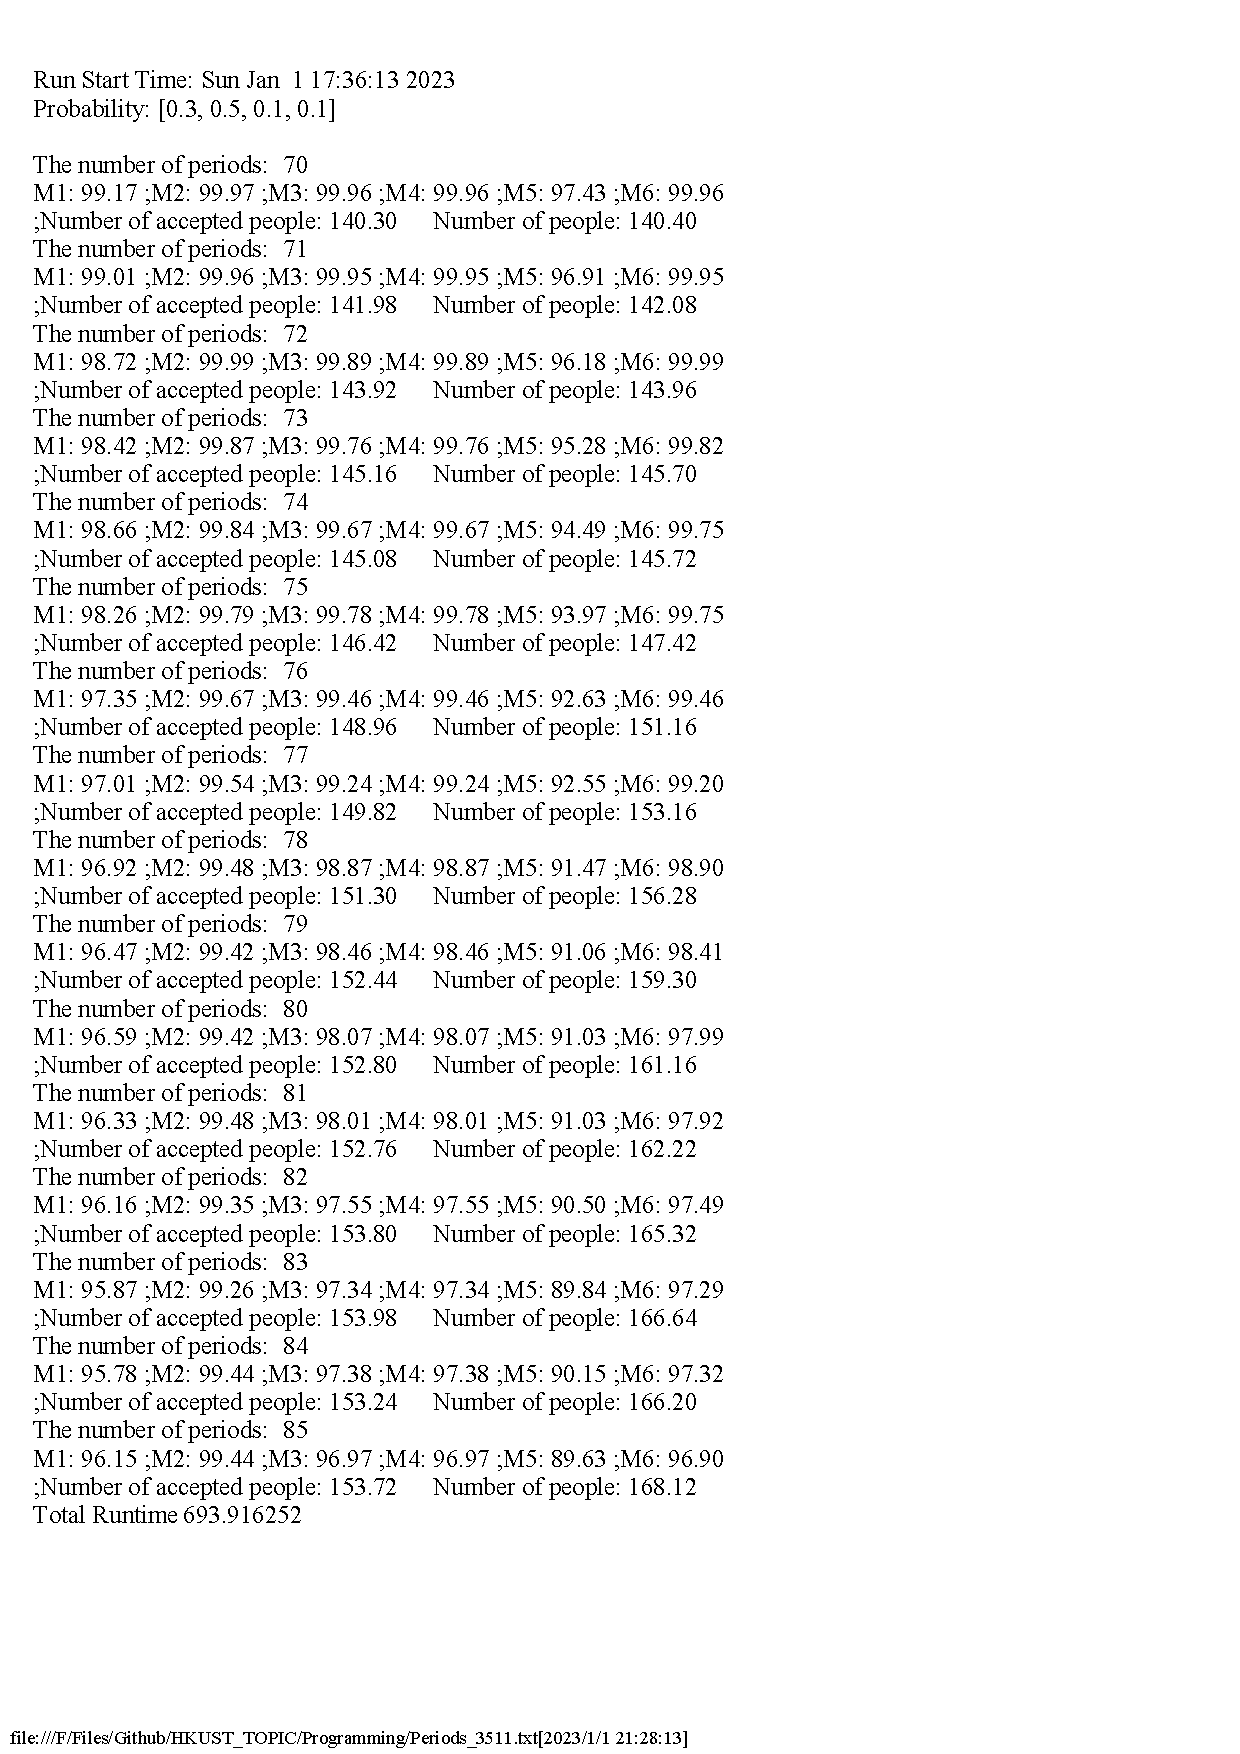
\includepdf{./Figures/Periods_3511.pdf}

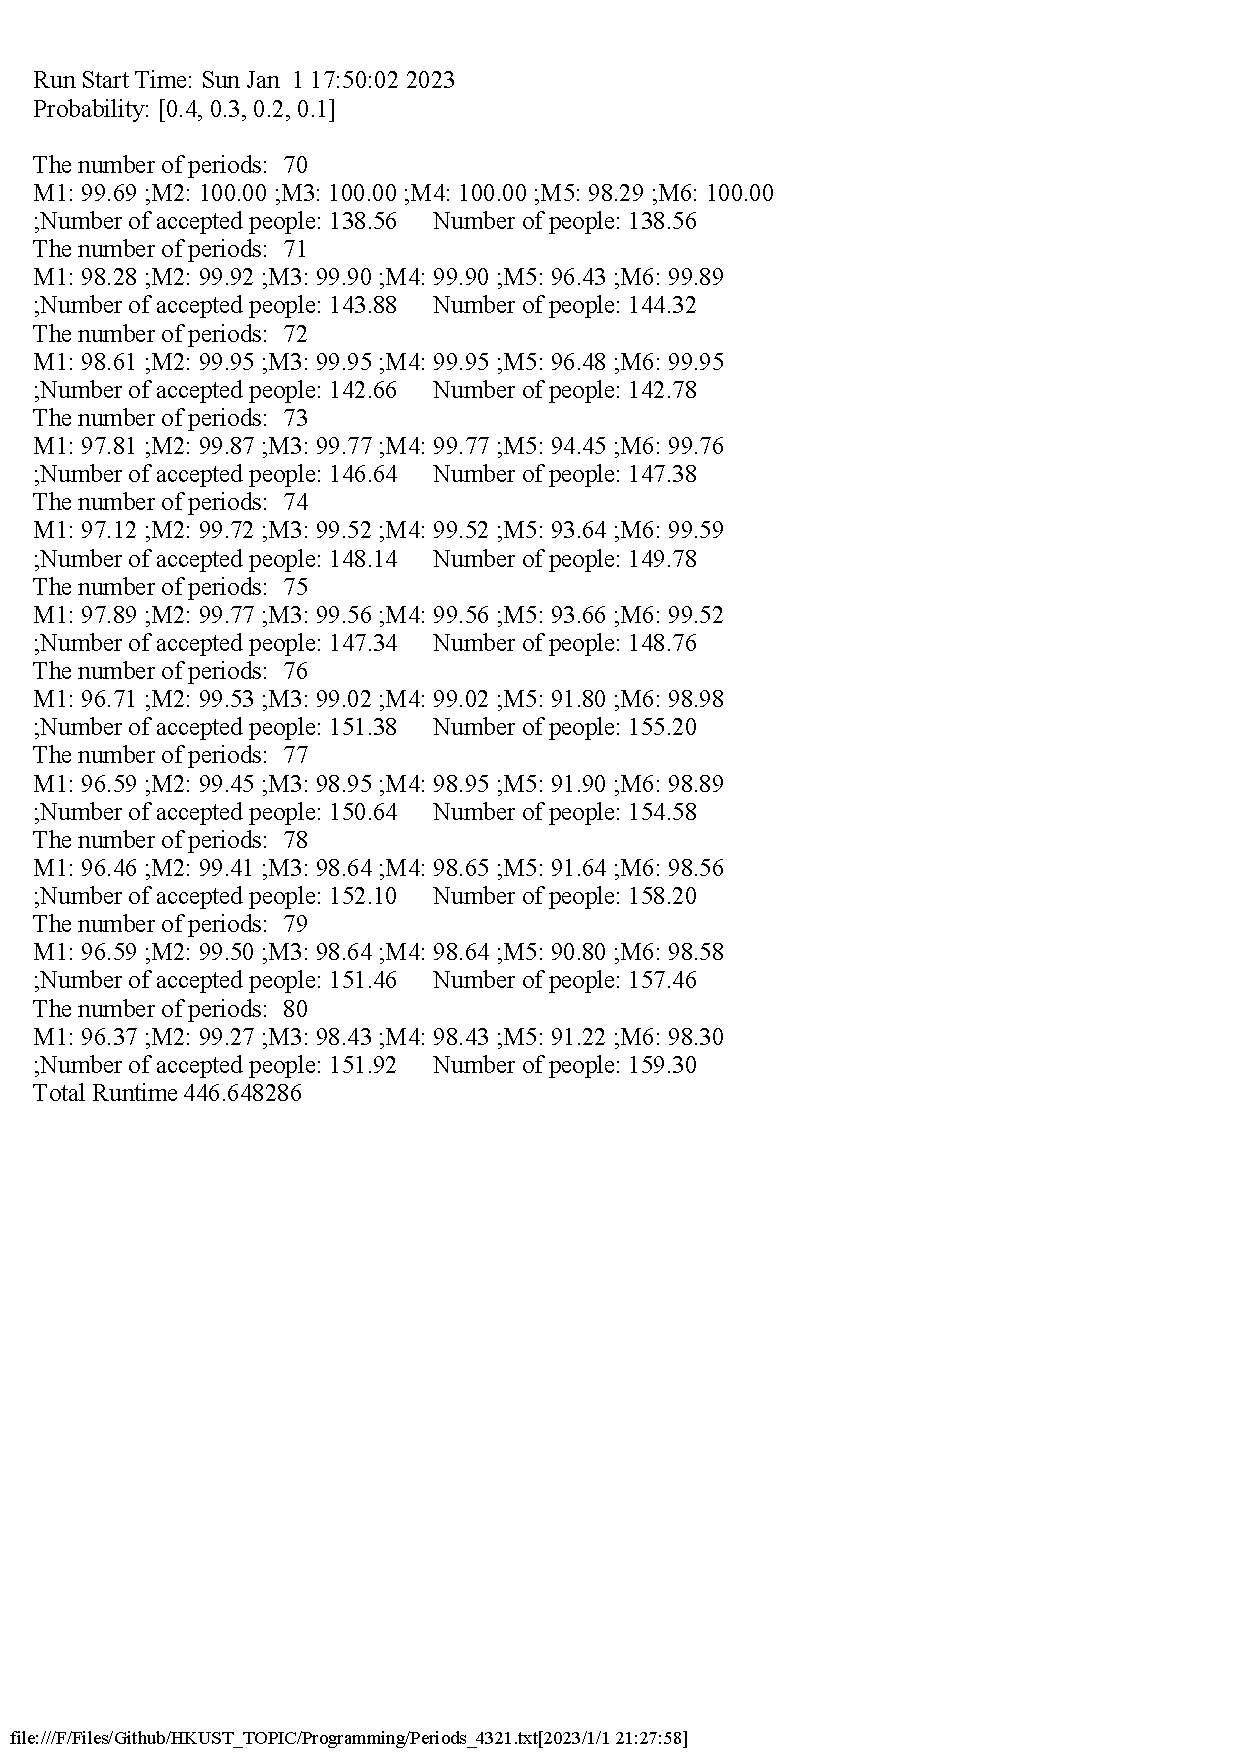
\includepdf{./Figures/Periods_4321.pdf}

T = 55-65, step size =1.

The expected number of period: 60
The expected number of demand(people): 150
Number of rows: 10
Number of seats each row: 21
Probabilities: $[0.25, 0.25, 0.25, 0.25]$.

Results: M1-M6, the number of accepted people, the number of total people.

We can find that the difference between the number of accepted people and the number of total people will increase with the period. 
% When the number of periods is small, the seats 

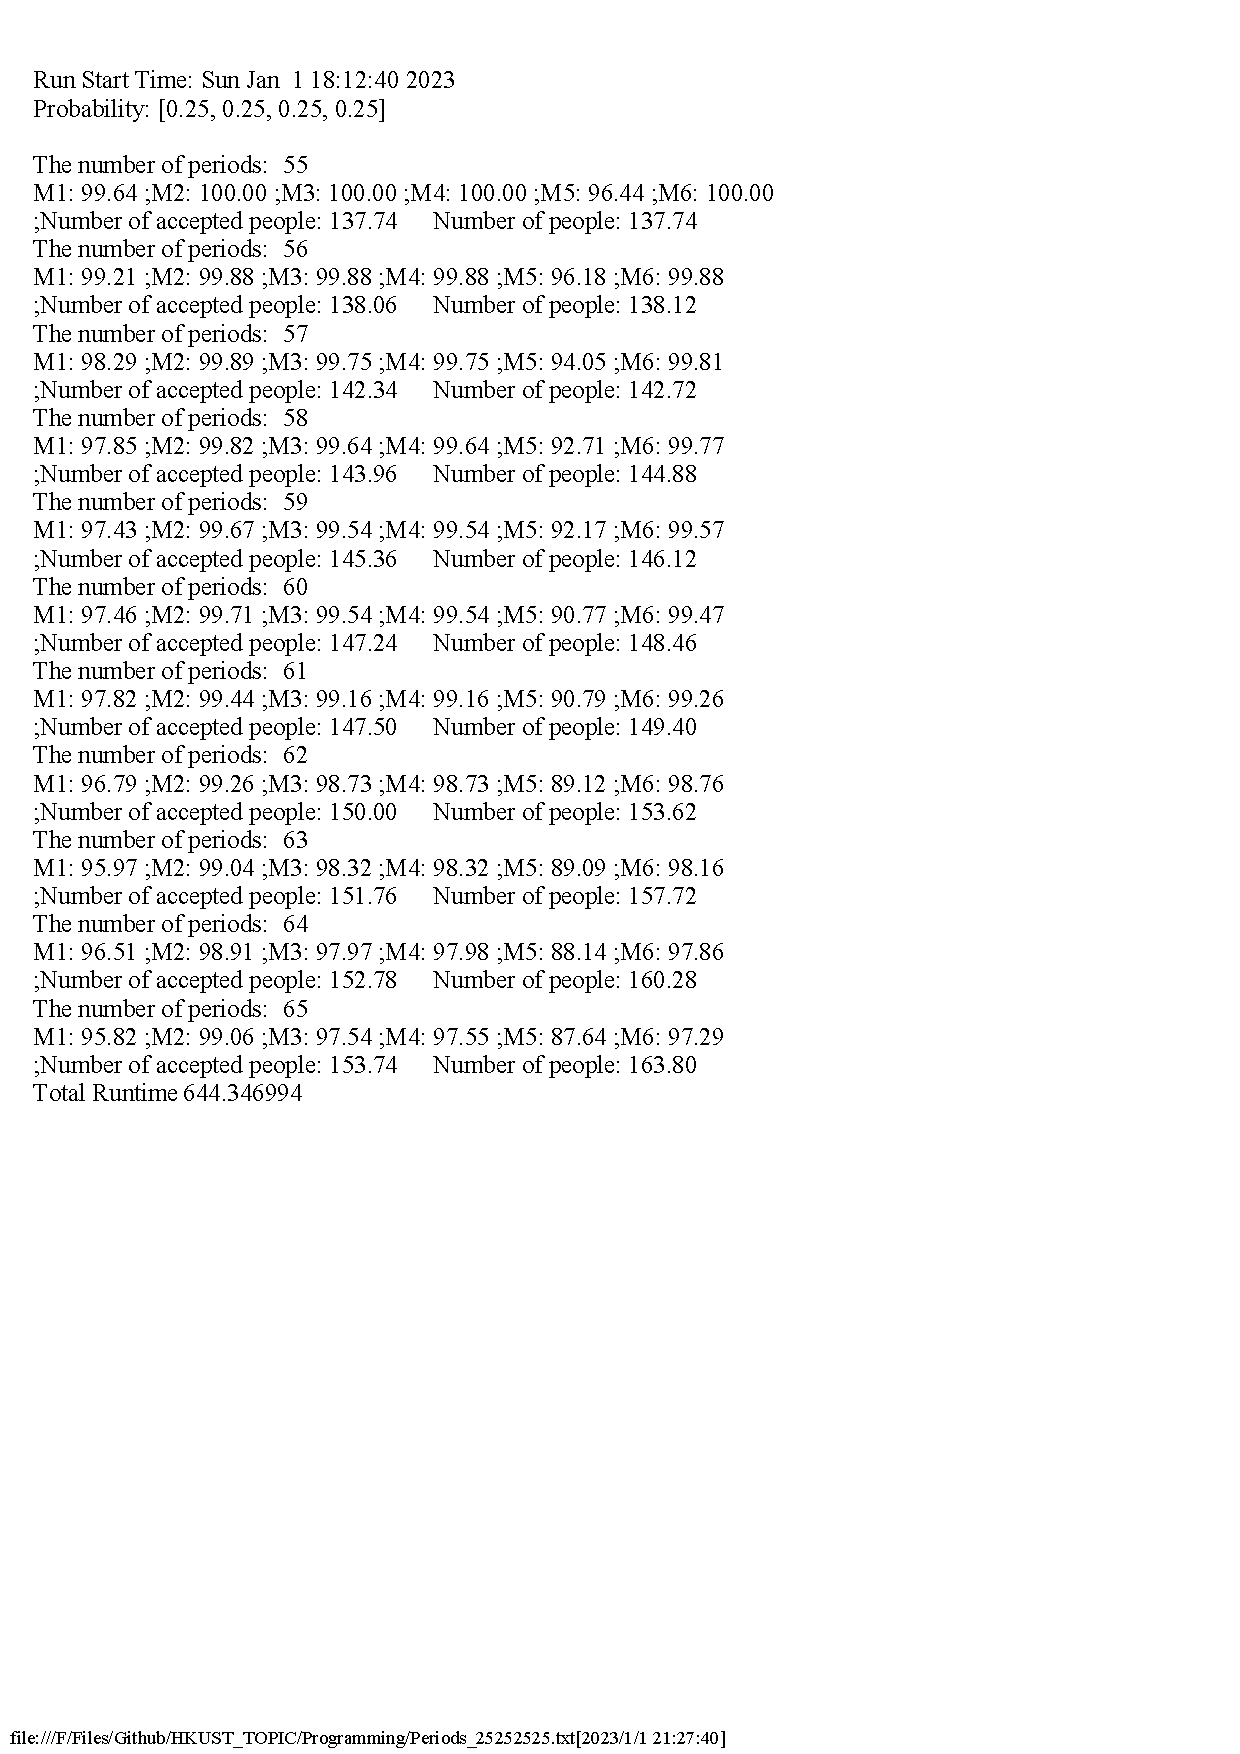
\includepdf{./Figures/Periods_25252525.pdf}

\subsection{Measurement}

Suppose a real scenario with a fixed sequence, $s^{r}$. Solving the following program can obtain the optimal value, $V_{s^{r}}$. (Offline)

Then the difference is $V_{s^{r}} - \text{our result}$.

WS(the value under wait-and-see policy with all possible scenarios)

EVPI(Expected Value of Perfect Information) = WS - the value of deterministic equivalent form

Regret.

\subsection{How to use the stochastic demand to solve the dynamic situation?}

\cite{bent2004scenario} this paper connects the stochastic and dynamic VRP.

Partially dynamic:

Scenario:

There is a reservation stage, we only decide to accept or reject.

After certain periods, there is a seat selection stage.



\subsection{How to give a balanced seat assignment}

Notice we only give the solution of how to assign seats for each row, but the order is not fixed.

In order to obtain a balanced seat assignment, we use a greedy way to place the seats.

Sort each row by the number of people. Then place the smallest one in row 1, place the largest one in row 2, the second smallest one in row 3 and so on. 

For each row, sort the groups in an ascending/descending order. In a similar way.

\newpage
